% Template for ICASSP-2013 paper; to be used with:
%          spconf.sty  - ICASSP/ICIP LaTeX style file, and
%          IEEEbib.bst - IEEE bibliography style file.
% --------------------------------------------------------------------------
\documentclass{article}
\usepackage{spconf,amsmath,graphicx}
\usepackage[utf8]{inputenc}
\usepackage{indentfirst}
\usepackage{url}

\makeatletter
\newcommand{\thickhline}{%
    \noalign {\ifnum 0=`}\fi \hrule height 1pt
    \futurelet \reserved@a \@xhline
}

% Example definitions.
% --------------------
\def\x{{\mathbf x}}
\def\L{{\cal L}}

% Title.
% ------
\title{Multipitch estimation using a PLCA-based model: Impact of partial user annotation} %and reassigned CQT-transform }
%
% Single address.
% ---------------
\name{Camila de Andrade Scatolini, Gaël Richard, Benoit Fuentes\thanks{This work was partially conducted within the project ANR-Edison 3D}}
\address{Institut Mines-Telecom, Télécom ParisTech, LTCI-CNRS\\
	37-39, rue Dareau - 75014 Paris - France\\
	}

\begin{document}
\ninept
%
\maketitle
%
\begin{abstract}
In this paper we investigate the merit of partial user annotation for music transcription using a PLCA-based model. The original algorithm, called Blind Harmonic Adaptive Decomposition (BHAD), provides an estimation of the polyphonic pitch content of the input signal in an entirely unsupervised manner. In this paper, we study how the performances of the BHAD algorithm can be further improved by involving a user by means of a partial annotation. This user input allows for a better model initialisation with adapted or learned spectral envelope models. Furthermore, it is studied how a fine control of the convergence rate of some parameters can better exploit this additional information. It is then shown that this partial annotation can bring an improvement of up to 3\% on the transcription of the remaining file.
\end{abstract}
%
\begin{keywords}
Multipitch estimation, PLCA, CQT, Semi-guided music transcription
\end{keywords}
%

\vspace{0.4cm}

\section{Introduction}
\label{sec:intro}
%Here we describe the interest of multipitch extraction and cite some of the important approaches (in particular probabilistic based). We then describe the interest of the BHAD model and describe in which ways it could be improved. Then mention main contributions (see below) and give the structure of the paper.

Multipitch estimation in musical recordings has received a great deal of attention in the last decade. This estimation task is known to be particularly challenging since a polyphonic music signal is typically composed of the
superposition of the sound waves produced by all instruments in the recording. In the context of music transcription,
multipitch extraction corresponds to the frame-by-frame estimation of all fundamental frequencies present in an audio signal.
%As multiple notes can be played simultaneously, the signal contains several $F_0$ at a given moment.
Two main issues arise in this estimation process :
the superposition of the different partials of each note played simultaneously can lead to ambiguity in the case of harmonically related sounds; and the total number of notes being played simultaneously is unknown.
Despite these difficulties, automatic multipitch estimation has many potential applications, including main melody extraction \cite{JS:SigMag2014, Durrieu2011, toosMelodyICASSP10}, cover song identification \cite{salamonVersionIDQBH-MMIR13} (detecting whether two recordings are different renditions of the same musical piece), or more generally music transcription \cite{HainsworthPhD}.

 %and much of the time these instruments play
%simultaneously. A typical polyphonic music signal results from the downmixing of multiple sound sources.
% a polyphonic music signal is composed of the
%superposition of the sound waves produced by all instruments in the recording, and much of the time these instruments play
%simultaneously.
% which can either be aperiodic (such as percussive drums) or quasi-periodic (as typical audio recording contains Music's sound environment is a complex result of the combination of multiple sound sources. For some tasks such as melody extraction, each musical instrument in a recording can be considered as one source. However, for tasks such as music transcription one can see each musical note as a different source. The sound of most instruments being a quasi-periodic signal and therefore formed by frequencies that are multiple of a fundamental frequency $F_0$, it is relevant to estimate this frequency, which is one of the major attributes that characterize a musical note.

\vspace{0.1cm}

Several methods were proposed in the literature for multipitch estimation \cite{Christensen2009_Morgan}. A number of approaches follows an iterative estimation strategy \cite{Klapuri2008} while others will aim at jointly estimating all fundamental frequencies \cite{Davy2006, Vincent2010_IEEE, Fuentes2012_EUSIPCO}. One class of techniques, which receives a sustained interest, exploits factorization models to represent the time-frequency representation of the audio signal as a sum of basic elements, called atoms.
%which in the most interesting case carry symbolic information.

\vspace{0.1cm}

A popular example of such decompositions is the non-negative matrix factorization (NMF), proposed by \cite{Lee99}, and widely used in music analysis \cite{Durrieu2011, Smaragdis03, Virtanen2008, Dessein10}.
In a probabilistic framework, Probabilistic Latent Component Analysis (PLCA) was shown to be particularly promising for audio signal analysis \cite{Benetos11c,Smaragdis06,Smaragdis08}.
PLCA is a probabilistic tool for non-negative data decomposition, where the time-frequency representation of an audio signal (e.g. the spectrogram $P(f,t)$) is modeled as the histogram of $J$ independent random variables $(f_j,t_j) \in \left[ 1,F \right] \times \left[ 1,T \right]$ distributed according to $P(f,t)$ where $f$ and $t$ respectively stands for frequency and time.

\vspace{0.1cm}

An algorithm called Blind Harmonic Adaptive Decomposition (BHAD) and its inherent model were presented in \cite{Fuentes2012_EUSIPCO, Fuentes2013_PhD} to better model real music signals. In this model, each musical note may present fundamental frequency and spectral envelope variations across repetitions. BHAD is an efficient algorithm and has obtained very good performances in an international evaluation campaign (ranked 2\textsuperscript{nd} in the MIREX-12 Multiple Fundamental Frequency Estimation \& Tracking task \cite{MIREX2012}).
%It uses the absolute value of the CQT of an audio signal as the time-frequency representation and its decompositions and parameters are found using the Expectation-Maximization (EM) algorithm.
The original approach is entirely unsupervised as most approaches in this framework which rely on prior generic information or signal models to obtain a semantically meaningful decomposition. It was shown in some controlled cases that improved performance can be obtained by integrating a learning stage or by adapting the pre-learned models using a multi-stage transcription strategy (see \cite{BenetosISMIR2014} for example) or by involving a user during the transcription process \cite{Kirchhoff13}, \cite{ozerov2012general}, \cite{BryanEtAl_2013_SourSepaOfPoly}.

\vspace{0.1cm}

In this paper, we have studied how the performance of the BHAD algorithm could be further improved by involving a user by means of a partial annotation (e.g. the user provides the transcription for the first ten seconds of the excerpt). This partial annotation allows for a better model initialisation with adapted or learned spectral envelope models. Furthermore, it is studied how a fine control of the convergence rate of some parameters can better exploit this additional information. It is then shown that this partial annotation can bring an improvement of up to 3\% on the transcription of the remaining file.  %Finally, using a reassigned CQT, which has better time-frequency resolution, the algorithm performances can improved even further.

%Main contributions compared to BHAD:
%\begin{enumerate}
%	\item Impact of better initialisation of spectral templates using a partial annotation of the music file
%	\item Interest of controlled convergence rate of the spectral templates (e.g. brake parameters)
	%\item Improved performances with a reassigned CQT
%\end{enumerate}
\vspace{0.1cm}
The paper is organised as follows. In the following section, we recall the main concepts of the original BHAD model. Three strategies for semi-guided transcription are then presented in section \ref{sec:semiguided}. Experiments and results are given and discussed in section \ref{sec:expres} and some conclusions are suggested in section \ref{sec:conc}.

\vspace{0.3cm}

\section{Original BHAD model}
\label{sec:Bhad}
The BHAD model is briefly described in this section. The reader is referred to \cite{Fuentes2012_EUSIPCO} for further details. BHAD relies on the framework of Probabilistic Latent Component Analysis (PLCA) which is a probabilistic tool for non-negative data analysis that offers a convenient way of designing spectrogram models and introducing priors on the corresponding parameters.
%we briefly describe here the BHAD model (it should be rather short but the concept should be understandable but the reader should be referred to Fuentes publications to fully understand. What is important is to describe all notations/concepts that will be useful later on in the paper).
In BHAD, the absolute value of the normalized constant-Q transform (CQT) of a signal is modeled as a probability distribution $P(f,t)$. By introducing a latent variable $c$, the signal is first decomposed as the sum of a polyphonic harmonic signal ($c=h$) and a noise signal ($c=n$):
%A latent variable $c$ is introduced in order to decompose the absolute value of the CQT of a music signal as the sum of a polyphonic harmonic signal ($c=h$) and a noise signal ($c=n$). The notation $P_h(.)$ and $P_n(.)$ is used for $P(.|c=h)$ and $P(.|c=n)$. The time-frequency distribution is then:
\begin{equation}
P(f,t) = P(c=h)P_h(f,t)+P(c=n)P_n(f,t),
\end{equation}
the notation $P_h(.)$ and $P_n(.)$ being used for $P(.|c=h)$ and $P(.|c=n)$.  We recall below the main concepts of the harmonic signal model. However, since the model of the noise component is left unchanged in this work, the reader is referred to \cite{Fuentes2012_EUSIPCO} for further details.
%\subsection{Noise signal}

%The noise signal is modeled as the convolution of a narrow-band window and a noise time-frequency distribution:

%\begin{equation}
%P_b(f,t) = \sum_i P_b(i,t)P_b(f-i).
%\end{equation}

\subsection{Polyphonic harmonic signal}
At time $t$, the polyphonic component $P_h(f,t)$ is modeled as a weighted sum of different harmonic spectra, each one having its own spectral envelope and fundamental frequency $i \in \left[ 0, I-1 \right]$. As the number of active notes is unknown, all possible fundamental frequencies are considered, with possibly zero weights:
%For a given instant $t$, the polyphonic component of the signal $P_h(f,t)$ is a weighted sum of the different harmonic spectra, each with its own spectral envelope and its own fundamental frequency $ i \in \left[ 0, I-1 \right] $. As we don't want to limit the number of notes present, we consider all the possible fundamental frequencies with probably zero weights:

\vspace{0.2cm}

\begin{equation}
P_h(f,t) = \sum_i P_h(i,t)P_h(f|i,t).
\end{equation}

$P_h(i,t)$ and $P_h(f|i,t)$ respectively represent the energy and the normalized harmonic spectra of a musical note of pitch $i$ at time $t$. We further model $P_h(f|i,t)$ as a linear combination of $Z$ fixed narrow-band harmonic kernels, sharing the same fundamental frequency $i$ and having energy concentrated on the $z^{th}$ harmonic:
%$P_h(i,t)$ is the note's energy at time $t$ and $P_h(f|i,t)$ is its normalized harmonic spectrum. Each harmonic spectrum is decomposed as a linear combination of $Z$ narrow-band harmonic kernels sharing the same fundamental frequency $i$ and having energy concentrated on the $z^{th}$ harmonic $P_h(f|z,i)$, weighted by its spectral envelope $P_h(z|i,t)$:

\begin{align}
P_h(f|i,t) & = \sum_z P_h(z|i,t)P_h(f|z,i) \\
P_h(f|i,t) & = \sum_z P_h(z|i,t)P_h(f-i|z).
\end{align}
%\begin{equation}
%\begin{array}{ll}
%P_h(f|i,t) & = \sum_z P_h(z|i,t)P_h(f|z,i) \\
%		   & = \sum_z P_h(z|i,t)P_h(f-i|z)
%\end{array}
%\end{equation}
In this last equation, an essential property of the CQT is exploited: a pitch modulation can be seen as a frequency shifting of the partials, and the kernel $P_h(f|z,i)$ can be deduced from a single template $P_h(\mu|z)$.
All parameters, except for the fixed kernels $P_h(\mu|z)$, are estimated with the Expectation-Maximization (EM) algorithm. By mean of a threshold applied on the time-frequency activations of harmonic spectra $P_h(i,t)$, it is then possible to estimate a MIDI pitch activations $\hat{A}(n,t)$ ($n$ representing MIDI notes) and thus address the problem of multipitch estimation.
%In this last equation it's used the main advantage of working with the CQT: a pitch modulation can be seen as a frequency shifting of the partials: $P_h(f|z,i) = P_h(f-i|z)$.

%Finally, the complete equation for the BHAD model is written as:

%\begin{equation}
%\begin{array}{ll}
%P(f,t) = & P(c=h)\sum_{i,z}P_h(i,t)P_h(z|i,t)P_h(f-i|z) \\
%& +P(c=n)\sum_i P_n(i,t)P_n(f-i)
%\end{array}
%\end{equation}

\subsection{Initialisation and priors}
\label{sec:init-prior}

%We want to estimate the following parameters: $\Lambda = \left \lbrace P(c), P_h(i,t), P_h(z|i,t), P_n(i,t) \right \rbrace$. Since this is an iterative optimization algorithm, the parameters initialisation plays a very important role in the quality of the decomposition.
Relevant initialisation can be seen as adding prior knowledge since parameters will likely converge toward a local optimum close to the initialisation.
%Therefore, in order to obtain a relevant decomposition, it is important that the parameters that will be estimated are well initialised.
In \cite{Fuentes2013_PhD} it is proposed that the spectral envelope coefficients $P_h(z|i,t)$ for the notes of pitch $i$ and time $t$ are initialised as a descending slope in $z$, as often for musical instruments an energy decay of the partials in function of their frequency is observed.

\vspace{0.1cm}

In order to even better account for relevant initialisation, it is also possible to use a ``brake" on the well initialised parameters as introduced in \cite{Fuentes_EUSCIPCO2014} (in our case the brake is applied to the spectral envelopes $P_h(z|i,t)$). By slowing down their convergence rate during EM algorithm, it is more likely that their values after convergence are close to their initialisation. In practice, the "brake" acts as a “steering wheel”, and then influences the direction in which the algorithm goes. The parameters may then converge towards a different local minimum than if no brake was used.
%$P_h(i,t)$ and $P_b(i,t)$ are initialised uniformly because it's not desirable to introduce a prior to the notes distribution or the noise energy.

\vspace{0.1cm}

In addition to relevant parameters initialisation, priors are used to integrate knowledge about the nature of the signals. A resemblance prior \cite{Fuentes2013_PhD} is applied to $P_h(z|i,t)$ for each pitch $i$ which allows to take into account that the spectral envelope of a note of given pitch slowly evolves over time. A sparseness prior is applied to the time-frequency activations $P_h(i,t)$ which helps to model the signal with the least amount of notes.

%Another concept is introduced in \cite{Fuentes2013_PhD} in order to guide the convergence of the parameters. A "brake" is applied to $P_h(z|i,t)$ and it considers that its true value is not far from the initialisation.

\vspace{0.3cm}


\section{Strategies for semi-guided transcription}
\label{sec:semiguided}

%We describe here the different strategies for semi-guided transcription :
%\begin{enumerate}
%	\item Manual annotation (what is annotated  10s vs 50\% of the file.. maybe we should only put the results for the ten first seconds.. to be discussed)
%	\item Strategies for initialisation of the non-annotated notes
%	\item Strategies for controlling the convergence rate of the annotated notes vs non-annotated notes
%\end{enumerate}

%\subsection{Manual annotation}
It is expected that involving the user in the transcription process should improve the overall transcription performances. In this paper, we evaluate a rather simple interaction process where the user has manually transcribed beforehand the first ten seconds of each processed musical recording. This partial transcription is then used to create initial templates of the spectral envelope $P(z|i,t)$ for each note of pitch $i$. If a note appears more than once in these first ten seconds, the template is obtained by averaging all occurrences of this given note for each kernel $z \in \left[1,Z\right]$. The transcription algorithm BHAD is then run as in the unsupervised case but with an improved initial estimation of, at least, some of the spectral envelopes $P(z|i,t)$.

\subsection{Strategies for initialisation of the non-annotated notes}

Unless if the music is highly repetitive, the note present in the first ten seconds only represent a subset of all notes played in the musical recording. The envelope templates of the remaining notes cannot be learned but still have to be initialised to some value before the BHAD algorithm is run. We evaluate below three strategies for initialising the templates of the remaining notes:

\begin{enumerate}
\item Keep the slope initialisation as in the original BHAD model: in this case we just consider the templates if they can be obtained from the learning phase, otherwise the spectral coefficients are initialised as a descending slope in $z$;
\item Copy the previous note template: the template of a note of given pitch $i_n$ is repeated for all subsequent notes of pitch $i \in [i_{n+1}, i_{p-1}]$ until another template is found (note of pitch $i_p$);
\item Interpolate neighbour notes' templates: the template for the notes of pitch $i \in [i_{n+1}, i_{p-1}]$ are obtained by linearly interpolating the templates of the notes of pitch $i_n$ and $i_p$ (on a dB scale).
\end{enumerate}

\subsection{Strategies for controlling the convergence rate of the annotated notes vs. non-annotated notes}

The goal of the learning phase using the partial user annotation is to improve the initial estimation of the spectral envelopes. If envelope parameters are well initialised, it is probable that their value are not very far from the ideal envelope templates.  It is then desirable to exploit this information to control the convergence rate of this parameter compared to other parameters of the models which are less well initialised. With BHAD, the convergence rate is controlled using the concept of brake (see section \ref{sec:init-prior} or \cite{Fuentes2012_EUSIPCO}). In the original BHAD model the convergence rate coefficient is equally applied to all note's templates to slow down their convergence compared to the other parameters of the model.  %However, even tough we have realized a better initialisation for the notes present in the learning phase, the other notes may not be as well initialised, for example, if we keep slope initialisation.
We suggest a modification of the BHAD model where the convergence rate coefficient $\beta_{brake}(n)$ now depends on the notes, so we can apply a stronger brake for the templates of the notes which were actually learned:

\begin{equation}
\beta_{brake}(n) = \left\{
\begin{array}{ll}
\beta_1, & \textrm{if }i_n\ \in \textrm{learning base} \\
\beta_0, & else
\end{array}
\right. , \textrm{ with } \beta_1 > \beta_0.
\end{equation}

%\pagebreak

\section{Experiments and Results}
\label{sec:expres}

\vspace{0.2cm}

\subsection{Database and evaluation metrics}

\vspace{0.1cm}

To assess the quality of the multipitch estimation provided by the algorithm, %it is necessary to have an evaluation database containing musical recordings and their corresponding ground truth.
its estimated activations $\hat{A}(n,t)$ are compared with the ground truth $A(n,t)$ and then evaluated in terms of F-measure. This measure combines the precision and recall measures in order to give a global index of the estimation's quality:

\vspace{0.1cm}

$$\mathcal{F}  = \frac{2\mathcal{P}\mathcal{R}}{\mathcal{P}+\mathcal{R}}.$$

\vspace{0.2cm}

The precision $\mathcal{P}$ indicates the ratio of activations correctly estimated by the total activations estimated while the recall $\mathcal{R}$ indicates the ratio of correctly estimated activations by all activations in the ground truth:

\vspace{0.1cm}

$$\mathcal{P}  = \frac{\sum_{n,t}\hat{A}(n,t)A(n,t)}{\sum_{n,t}\hat{A}(n,t)}, \quad \mathcal{R}  = \frac{\sum_{n,t}\hat{A}(n,t)A(n,t)}{\sum_{n,t}A(n,t)}.$$

\vspace{0.2cm}

We used the QUASI-Transcription database elaborated under the QUAERO\footnote{\url{http://www.quaero.org}} project and \cite{Fuentes2013_PhD}. It contains pieces of contemporary music, belonging to different genres with a high degree of polyphony (see table \ref{tab:quaero} which details the characteristics of each song in the database). The instruments are a mixture of virtual (e.g. synthetic) and acoustic instruments. For virtual instruments, transcripts were obtained from the corresponding MIDI file, while for acoustic instruments, they were manually transcribed.
The database is split in two : a training database built from the first 10s of each file and a test database  which gathers the remaining part of all songs. All results are given on the test database.

\begin{table}[htb]
\centering
\begin{tabular}{lcccc}
\\
\hline
Song name & Duration & $\#$ inst./notes & Poly. (mean/max) \\\hline
RockSong & 01'14'' & 9/1039 & 3.9/10 \\
Choir & 01'11'' & 4/224 & 3.4/4 \\
Filter & 01'19'' & 19/2418 & 5.9/11 \\
Unison & 01'17'' & 6/561 & 5.6/9 \\
Accelerando & 01'49'' & 3/1046 & 2.3/6 \\
\end{tabular}
\caption{QUASI-Transcription database}
\label{tab:quaero}
\end{table}

\vspace{0.3cm}

\subsection{Experiments and Results}

%\begin{enumerate}
%	\item Comparaison with and without 10s annotation
%	\item Comparaison of the different initialisation strategies
%	\item Impact of convergence rate (Brake coefficient) adaptation
%	\item Impact of using a reassigned CQT
%\end{enumerate}

We compared the algorithm performances for the unsupervised and semi-guided approaches for all combination of priors (sparseness - S and resemblance - R) and guided parameters convergence (brake - B), including the case where no prior or brake was used (NO). The initialisation for the unsupervised approach is the one that is proposed in \cite{Fuentes2013_PhD}: for each note of pitch $i$ and time $t$ the spectral envelope is initialised as a descending slope in $z$. In the semi-guided approach, the spectral envelopes are initialised either by the templates obtained in the learning phase or one of the three strategies of initialisation for the non-annotated notes (slope, copy and interpolation).


\begin{figure}[!ht]
\begin{minipage}[b]{1.0\linewidth}
  \centering
  \centerline{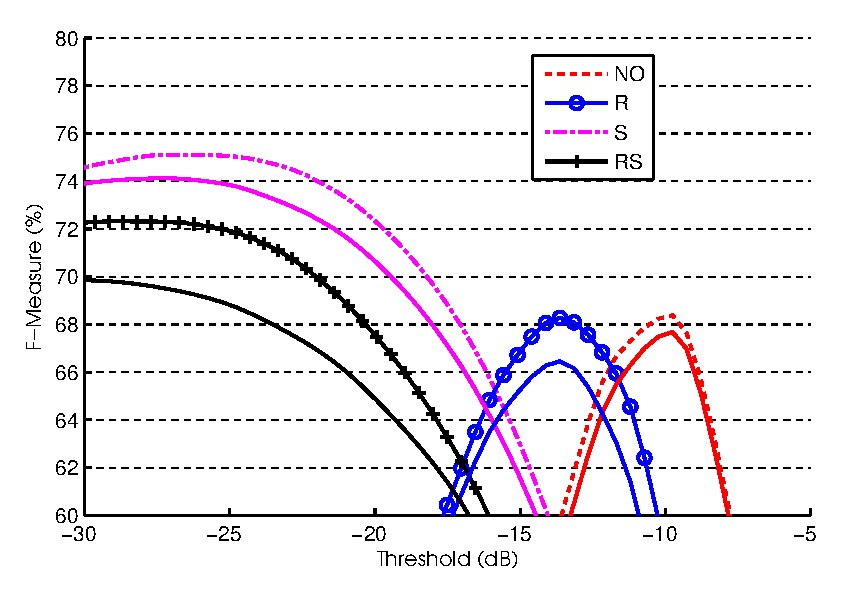
\includegraphics[width=8.5cm, height=6.7cm]{figures/finalnobrake.eps}}
\end{minipage}
\caption{Comparison of the mean F-Measure for all 5 songs in the database in function of the threshold applied on the time-frequency activations $P_h(i,t)$ for the semi-guided approach with slope initialisation for the non-annotated notes (symbols) and the unsupervised approach (continuous line) for all combinations of priors without brake coefficients.}
\label{fig:fxt-nobrake}
\end{figure}

\vspace{0.2cm}

The results of these tests are shown in Figure \ref{fig:fxt-nobrake} and Table \ref{tab:init}. The best results for the options without the brake (e.g. options NO, S, R and SR), obtained with the semi-guided approach with slope initialisation of the non-annotated notes are presented in Figure \ref{fig:fxt-nobrake} for a range of detection threshold values. In this Figure, the continuous lines correspond to the unsupervised approach and the lines with symbols correspond to the user-guided approach.  It can be noticed that the user inputs bring a systematic performance increase regardless of the detection threshold value.

The table gathers the results obtained \textit{a posteriori}, that is with a choice of the detection threshold that maximises the algorithm's performance for each combination of priors and brake on the entire test database.

\vspace{0.2cm}

\begin{table}[htb]
\begin{tabular}{ccccc}
\hline
\textbf{Options} & \textbf{Unsupervised} & \multicolumn{3}{c}{\textbf{Semi-Guided}} \\\thickhline
 & & Slope & Copy & Interpolation \\\hline
 NO  & 67.68 &	 \textbf{68.38} &	 65.00 &	 43.68 \\
 S   & 73.91 &     \textbf{75.07} &	 71.44 &	 52.07 \\
 R   & 66.46 &	 \textbf{68.28} &	 64.13 &	 47.05 \\
 RS  & 69.51 &	 \textbf{72.30} &	 67.60 &	 52.35 \\ \hline
 B   & 77.85 &	 \textbf{78.63} &	 75.88 &	 50.90 \\
 SB  & 74.64 &	 \textbf{76.54} &	 72.47 &	 45.68 \\
 RB  & 77.39 &	 \textbf{79.49} &	 73.89 &	 50.79 \\
 RSB & 74.85 &	 \textbf{77.02} &	 70.52 & 	 47.00  \\\thickhline
\end{tabular}
\caption{Mean F-Measure for the semi-guided and unsupervised approaches, considering the different initialisations of the non-annotated notes (Slope, Copy and Interpolation) and the different options of the BHAD algorithm : sparseness (S) and resemblance (R) priors, convergence rate parameter (brake B); Option NO refers to no prior and no brake.}
\label{tab:init}
\end{table}


The results in Table \ref{tab:init} show that the use of the semi-guided approach with slope initialisation of the non-annotated notes increases the mean F-measure between $1\%$ and $3\%$. This table also shows that, for the copy initialisation the F-measure decreases around $2\%$ or even $4\%$ when compared to the unsupervised approach. This degradation of the results is even more important in the case of the interpolated initialisation. We note that, in general, the gain in terms of F-measure is greater for the case where the brakes are used for guiding the convergence of the parameters.

Using copied spectral envelope templates as initialisation for non-annotated notes introduces a bias in the estimation task by assuming that all the notes are present. As the algorithm starts with a calculated spectral envelope instead of a simple slope in $z$, it causes the algorithm to assume that these notes are present (smaller precision when compared to the unsupervised approach). Templates obtained by interpolating adjacent notes presented the worst results since in this case besides introducing the copy initialisation bias, the templates were not really learned as in the previous case.

Regarding the different strategies for controlling the convergence rate of the annotated notes, we tested two cases:

\begin{enumerate}
\item The brake coefficient is only applied to annotated notes ($\beta_0=0$);
\item The same brake coefficient used in the previous tests ($\beta_0=10$) is applied to the non-annotated notes but a greater coefficient is applied to the annotated notes.
\end{enumerate}
Similarly to the previous experiment, the results are given in Table \ref{tab:brake} for all options with a choice \textit{a posteriori} of the detection threshold. The best results considering a different convergence rate of the calculated spectral envelope templates ($\beta_0=10$ and $\beta_1=20$) and  slope initialisation of the non-annotated notes for the semi-guided approach are presented in Figure \ref{fig:fxt-brake}.


\begin{table}[htb]
\begin{tabular}{ccccc}
\hline
\textbf{Option} & \textbf{No brake} & \multicolumn{3}{c}{\textbf{Brake annotated notes ($\beta_0=0$)}} \\\thickhline
& $\beta_{0,1}=0$ & $\beta_1=0.1$ & $\beta_1=1$ & $\beta_1=10$ \\\hline
B	& \textbf{68,38} &	68,25	& 66,43 &	 62,93 \\
SB	& \textbf{75,07} &	 74,84 	& 74,29 &	 72,74 \\
RB	& 68,28 & 	 68,53 	& \textbf{69,20} & 	 69,16 \\
RSB	& 72,30 &	 72,35 	& 72,53 &	 \textbf{72,66} \\\thickhline
\end{tabular}
  \centerline{(a) Brake coefficient only for annotated notes.}
\\
\\%
\vspace{0.1cm}

\centering
 \begin{tabular}{ccccc}
 \hline
\textbf{Option} & \textbf{Even brake} & \multicolumn{3}{c}{\textbf{Brake all notes ($\beta_0=10$)}} \\\thickhline
& $\beta_{0,1}=10$ & $\beta_1=10.1$ & $\beta_1=11$ & $\beta_1=20$ \\\hline
B	& 78,63 &	78,63 & \textbf{78,66} &	\textbf{78,66} \\
SB	& 76,54 &	 76,54 &	\textbf{76,55} &	\textbf{76,55} \\
RB	& 79,49 &	 79,49 &	79,51 &	\textbf{79,61} \\
RSB	& 77,02 &	 77,02 &	\textbf{77,03} &	76,98 \\\thickhline
\end{tabular}
  \centerline{(b) Brake coefficient greater for annotated notes.}\medskip
\caption{Mean F-Measure considering the different strategies for controlling the convergence rate of the annotated notes and the different options of the BHAD algorithm (priors).}
\label{tab:brake}
\end{table}

\begin{figure}[!ht]
\begin{minipage}[b]{1.0\linewidth}
  \centering
  \centerline{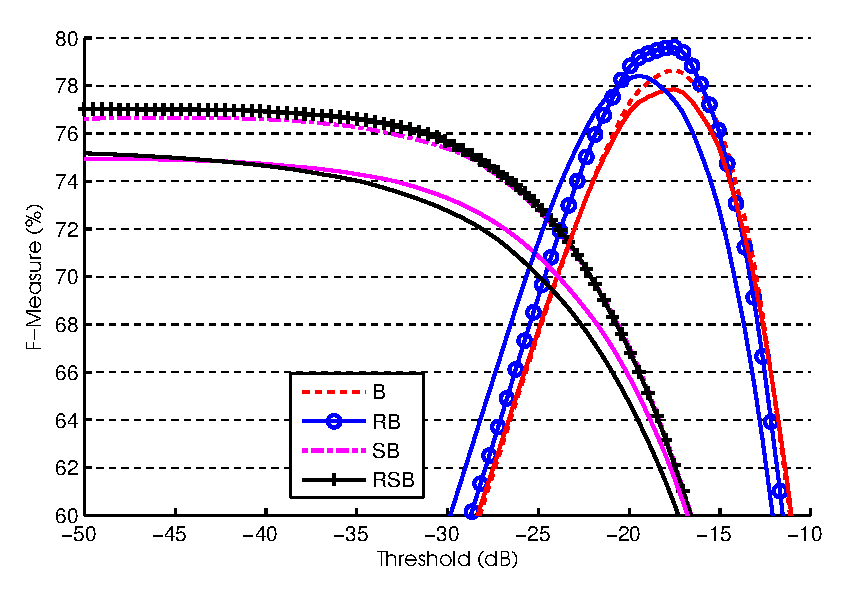
\includegraphics[width=8.5cm,height=6.7cm]{figures/finalbrake.eps}}
\end{minipage}
\caption{Mean F-Measures as a function of the threshold applied on the time-frequency activations $P_h(i,t)$ for the semi-guided approach with slope initialisation for the non-annotated notes (symbols) and the unsupervised approach (continuous line) for all combinations of priors with brake coefficients with $\beta_1=20$ for annotated notes and $\beta_0=10$ elsewhere.}
\label{fig:fxt-brake}
\end{figure}


The results in Table \ref{tab:brake}.(a) show that when we apply the brake coefficient only for the annotated notes, the improvement of the F-measure depends on the considered priors. In particular, when the resemblance prior is used we note that the results improve up to $1\%$ by using the brake coefficient for the annotated notes. However, the results in Table \ref{tab:brake}.(b) (where the brake coefficient is used for all notes) show that there is little interest to use a more restrictive convergence rate for annotated notes compared to the one used for non-annotated notes (a maximum of $0.1\%$ increase in F-measure is observed).


\section{Conclusion}
\label{sec:conc}

As highlighted in an international evaluation campaign, the original BHAD algorithm is a powerful approach for multipitch extraction of music recordings. Since it is entirely unsupervised, it relies on a very generic model for the initial estimation of the notes spectral templates.
It is shown in this paper that a substantial gain in performance can be obtained with the introduction of a learning step with a partial user annotation of even a small part of the song (first $ 10$ seconds). This partial annotation allows for a better initialisation of the model parameters by using learned spectral envelope models for the notes that are present in the annotation. The experiments have shown that this partial annotation can lead to an improvement of up to $3\%$ in terms of F-measure in a task of multipitch estimation. It was also shown that a fine control of the convergence rate of these learned models helps to better exploit this additional information.

Future work will be dedicated to the investigation of alternative strategies for optimizing the user annotation effort, for example by rather annotating specific parts of the song such as the main melody, the bass line or one of the chorus of the song. Another strategy would involve the user in a more iterative way for example letting the user transcribe the segments where the algorithm is the least confident.


%\vfill\pagebreak
%\clearpage

\bibliographystyle{IEEEbib}
\bibliography{refs}

\end{document}

%Major headings, for example, "1. Introduction", should appear in all capital
%letters, bold face if possible, centered in the column, with one blank line
%before, and one blank line after. Use a period (".") after the heading number,
%not a colon.
%
%\subsection{Subheadings}
%\label{ssec:subhead}
%
%Subheadings should appear in lower case (initial word capitalized) in
%boldface.  They should start at the left margin on a separate line.
%
%\subsubsection{Sub-subheadings}
%\label{sssec:subsubhead}
%
%Sub-subheadings, as in this paragraph, are discouraged. However, if you
%must use them, they should appear in lower case (initial word
%capitalized) and start at the left margin on a separate line, with paragraph
%text beginning on the following line.  They should be in italics.
%
%\section{PRINTING YOUR PAPER}
%\label{sec:print}
%
%Print your properly formatted text on high-quality, 8.5 x 11-inch white printer
%paper. A4 paper is also acceptable, but please leave the extra 0.5 inch (12 mm)
%empty at the BOTTOM of the page and follow the top and left margins as
%specified.  If the last page of your paper is only partially filled, arrange
%the columns so that they are evenly balanced if possible, rather than having
%one long column.
%
%In LaTeX, to start a new column (but not a new page) and help balance the
%last-page column lengths, you can use the command ``$\backslash$pagebreak'' as
%demonstrated on this page (see the LaTeX source below).
%
%\section{PAGE NUMBERING}
%\label{sec:page}
%
%Please do {\bf not} paginate your paper.  Page numbers, session numbers, and
%conference identification will be inserted when the paper is included in the
%proceedings.
%
%\section{ILLUSTRATIONS, GRAPHS, AND PHOTOGRAPHS}
%\label{sec:illust}
%
%Illustrations must appear within the designated margins.  They may span the two
%columns.  If possible, position illustrations at the top of columns, rather
%than in the middle or at the bottom.  Caption and number every illustration.
%All halftone illustrations must be clear black and white prints.  Colors may be
%used, but they should be selected so as to be readable when printed on a
%black-only printer.
%
%Since there are many ways, often incompatible, of including images (e.g., with
%experimental results) in a LaTeX document, below is an example of how to do
%this \cite{Lamp86}.
%
%\section{FOOTNOTES}
%\label{sec:foot}
%
%Use footnotes sparingly (or not at all!) and place them at the bottom of the
%column on the page on which they are referenced. Use Times 9-point type,
%single-spaced. To help your readers, avoid using footnotes altogether and
%include necessary peripheral observations in the text (within parentheses, if
%you prefer, as in this sentence).
%
%% Below is an example of how to insert images. Delete the ``\vspace'' line,
%% uncomment the preceding line ``\centerline...'' and replace ``imageX.ps''
%% with a suitable PostScript file name.
%% -------------------------------------------------------------------------
%\begin{figure}[htb]
%
%\begin{minipage}[b]{1.0\linewidth}
%  \centering
%  \centerline{\includegraphics[width=8.5cm]{image1}}
%%  \vspace{2.0cm}
%  \centerline{(a) Result 1}\medskip
%\end{minipage}
%%
%\begin{minipage}[b]{.48\linewidth}
%  \centering
%  \centerline{\includegraphics[width=4.0cm]{image3}}
%%  \vspace{1.5cm}
%  \centerline{(b) Results 3}\medskip
%\end{minipage}
%\hfill
%\begin{minipage}[b]{0.48\linewidth}
%  \centering
%  \centerline{\includegraphics[width=4.0cm]{image4}}
%%  \vspace{1.5cm}
%  \centerline{(c) Result 4}\medskip
%\end{minipage}
%%
%\caption{Example of placing a figure with experimental results.}
%\label{fig:res}
%%
%\end{figure}
%
%
%% To start a new column (but not a new page) and help balance the last-page
%% column length use \vfill\pagebreak.
%% -------------------------------------------------------------------------
%%\vfill
%%\pagebreak
%
%\section{COPYRIGHT FORMS}
%\label{sec:copyright}
%
%You must submit your fully completed, signed IEEE electronic copyright release
%form when you submit your paper. We {\bf must} have this form before your paper
%can be published in the proceedings.
%
%\section{RELATION TO PRIOR WORK (NEW)}
%\label{sec:prior}
%
%The text of the paper should contain discussions on how the paper's
%contributions are related to prior work in the field. It is important
%to put new work in  context, to give credit to foundational work, and
%to provide details associated with the previous work that have appeared
%in the literature. This discussion may be a separate, numbered section
%or it may appear elsewhere in the body of the manuscript, but it must
%be present.
%
%You should differentiate what is new and how your work expands on
%or takes a different path from the prior studies. An example might
%read something to the effect: "The work presented here has focused
%on the formulation of the ABC algorithm, which takes advantage of
%non-uniform time-frequency domain analysis of data. The work by
%Smith and Cohen \cite{Lamp86} considers only fixed time-domain analysis and
%the work by Jones et al \cite{C2} takes a different approach based on
%fixed frequency partitioning. While the present study is related
%to recent approaches in time-frequency analysis [3-5], it capitalizes
%on a new feature space, which was not considered in these earlier
%studies."
%
%\vfill\pagebreak
%
%\section{REFERENCES}
%\label{sec:refs}
%
%List and number all bibliographical references at the end of the
%paper. The references can be numbered in alphabetic order or in
%order of appearance in the document. When referring to them in the
%text, type the corresponding reference number in square brackets
%as shown at the end of this sentence \cite{C2}. \textbf{An
%additional final page (the fifth page, in most cases) is allowed,
%but must contain only references to the prior literature.}
%
%% References should be produced using the bibtex program from suitable
%% BiBTeX files (here: strings, refs, manuals). The IEEEbib.bst bibliography
%% style file from IEEE produces unsorted bibliography list.
%% -------------------------------------------------------------------------
